\documentclass[tikz,border=20pt]{standalone}
\usetikzlibrary{calc}

\begin{document}
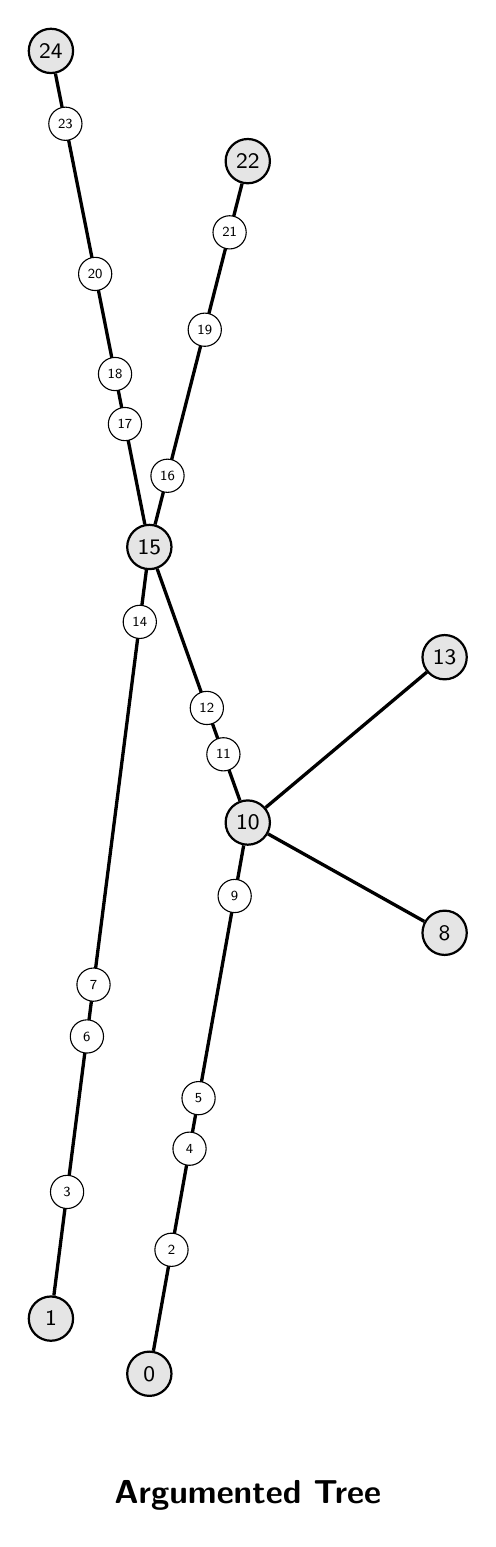
\begin{tikzpicture}[
    y=0.7cm, x=2.5cm,
    crit node/.style={circle, draw=black, fill=gray!20, thick, inner sep=1pt, minimum size=16pt, font=\sffamily\footnotesize},
    reg node/.style={circle, draw=black, fill=white, inner sep=0.5pt, minimum size=12pt, font=\sffamily\tiny},
    main edge/.style={very thick, draw=black}
]

% 关键点 (所有极值与鞍点)
\node[crit node] (C24) at (0, 24) {24};
\node[crit node] (C22) at (1, 22) {22};
\node[crit node] (C15) at (0.5, 15) {15};
\node[crit node] (C13) at (2, 13) {13};
\node[crit node] (C10) at (1, 10) {10};
\node[crit node] (C8)  at (2, 8) {8};
\node[crit node] (C1)  at (0, 1) {1};
\node[crit node] (C0)  at (0.5, 0) {0};

% 连线与普通节点填充
\draw[main edge] (C15) -- (C24);
\foreach \v in {17, 18, 20, 23} \path (C15) -- (C24) node[pos={(\v-15)/(24-15)}, reg node] {\v};

\draw[main edge] (C15) -- (C22);
\foreach \v in {16, 19, 21} \path (C15) -- (C22) node[pos={(\v-15)/(22-15)}, reg node] {\v};

\draw[main edge] (C1) -- (C15);
\foreach \v in {3, 6, 7, 14} \path (C1) -- (C15) node[pos={(\v-1)/(15-1)}, reg node] {\v};

\draw[main edge] (C10) -- (C15);
\foreach \v in {11, 12} \path (C10) -- (C15) node[pos={(\v-10)/(15-10)}, reg node] {\v};

\draw[main edge] (C10) -- (C13); 

\draw[main edge] (C8) -- (C10); 

\draw[main edge] (C0) -- (C10);
\foreach \v in {2, 4, 5, 9} \path (C0) -- (C10) node[pos={(\v-0)/(10-0)}, reg node] {\v};

\node[font=\sffamily\bfseries\large] at (1, -2.2) {Argumented Tree};

\end{tikzpicture}
\end{document}
